\documentclass{beamer}
\usepackage[utf8]{inputenc}

\usetheme{Madrid}
\usecolortheme{beaver}

\title[About Beamer]{A sample class on beamer}
\subtitle{in sleepy mode}

\author[L.M. and C.R.]{Lionel Messi \inst{1} \and Christiano Ronaldo\inst{2}}

\institute[BUET]
{
\inst{1}
Department of Physics\\
BUET\\
\inst{2}
Department of Mathematics\\
BUET\\
}
\date{\today}


\AtBeginSection
{
\begin{frame}{We are going to start}
    \tableofcontents[currentsection]
\end{frame}
}

\begin{document}
\titlepage

\begin{frame}{Table of Contents}
    \tableofcontents
\end{frame}

\section{Introduction}
\begin{frame}{Introduction}
This is our first slide.
\end{frame}
\section{Animation}
\begin{frame}{Sample Animation}
\begin{enumerate}
    \item CSE 300
    \begin{itemize}
        \item Very Simple
        \item So Easy
    \end{itemize} \pause
    \item CSE 305 \pause
    \item CSE 309
\end{enumerate}
    
\end{frame}


\begin{frame}{Sample Animation in another way}
\setbeamercovered{dynamic}
\begin{enumerate}
    \item CSE 300
    \begin{itemize}
        \item<2-> Very Simple
        \item<3-> So Easy
    \end{itemize} 
    \item<4-> CSE 305 
    \item<5-> CSE 309
\end{enumerate}
    
\end{frame}

\begin{frame}{Table and Animation in Beamer}
\setbeamercovered{dynamic}
    \begin{center}
        \begin{tabular}{|c|c|c|}
            \hline
            Table & X & Y  \\
            \hline
            A & \onslide<2->{1} & \onslide<3->{0} \\
            \hline
            B & \onslide<4->{0} & \onslide<5->{1}\\
            \hline
        \end{tabular}
    \end{center}
\end{frame}
\section{Column}
\begin{frame}{Columns}
\begin{columns}
\column{0.5\textwidth}
\begin{center}
        \begin{tabular}{|c|c|c|}
            \hline
            Table & X & Y  \\
            \hline
            A & \onslide<2->{1} & \onslide<3->{0} \\
            \hline
            B & \onslide<4->{0} & \onslide<5->{1}\\
            \hline
        \end{tabular}
    \end{center}
\column{0.5\textwidth}
This is a sample Truth Table.
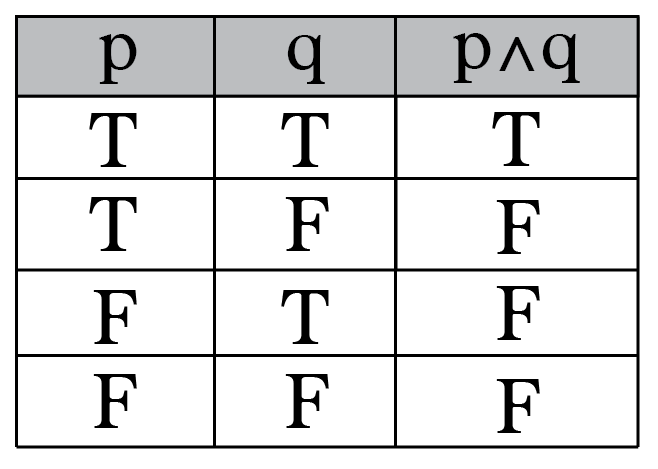
\includegraphics[height=2cm]{truth.png}
\end{columns}
    
\end{frame}

\section{Design and Formatting}
\begin{frame}{Design}
    \begin{block}{Sleep}
    Donot \textcolor<3>{green}{Sleep}!
    \end{block}
    
    \begin{alertblock}{Alert}
    This is to \textbf<2>{alert} you! Donot talk in the class!
    \end{alertblock}
    
    \begin{example}
    As an example I am not talking or sleeping.
    \end{example}
\end{frame}


\end{document}
